\section{On-Screen Appearance Requirements}
{
\begin{figure}
\centering
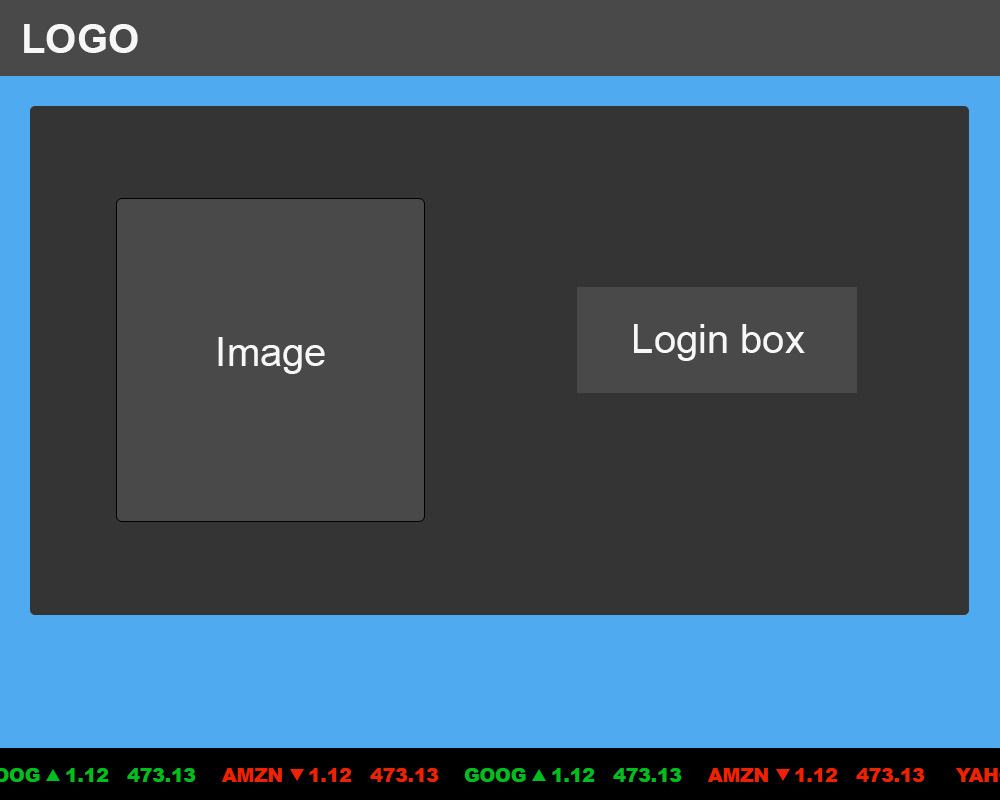
\includegraphics[width=5.5in]{./img/mock/loginmock.jpg}
\caption{Basic on screen requirements of login page}
\label{ui:mockup}
\end{figure}
}

There are a few on screen requirements that will be universal to the entire site:\\
\renewcommand\arraystretch{2}
\begin{longtable}{|p{0.6in}|p{4.6in}|}
\hline
{\large \color{color1}Identifier}&{\large \color{color1}Requirement} \\ \hline

OSR-1& Every page has a scrolling ticker across the bottom of the page to update the user
on stock movement. \\ \hline

OSR-2& Every page, with the exception of the login page, will have
navigational links across the top, the user's username and their current position in
the leaderboard. \\ \hline

\end{longtable}


There are also the following requirements for specific pages:\\

\renewcommand\arraystretch{2}
\begin{longtable}{|p{0.6in}|p{4.6in}|}
\hline
{\large \color{color1}Identifier}&{\large \color{color1}Requirement} \\ \hline

OSR-3&  A custom 404 not found page will be displayed to a user when they try to  access
a URL/URI that doesn't exist or is not designed for them to be accessing. \\ \hline

OSR-4& On the portfolio page users will find currently owned stocks, charts and graphs,
trade transcations, and a news feed. \\ \hline

OSR-5&  The leaderboard view will contain users ranked by the top networth from their
respective portfolios. \\ \hline

OSR-6&  The login page will present the user with login icons representing the service
they can use to log into our system, eg: google+, facebook, etc. \\ \hline

\end{longtable}

